
\chapter{Thermo-mechanical coupling} \label{ssn_thermo_mechanical_coupling}

Coupling between the momentum-balance models described in Chapter \ref{ssn_momentum_and_mass_balance} and the energy-balance model of Chapter \ref{ssn_internal_energy_balance} -- referred to as \index{Thermo-mechanical coupling} \emph{thermo-mechanical coupling} (TMC) -- is accomplished here via fixed-point iteration, a process which generates approximations of velocity $\rankone{u}$, pressure $p$, and energy $\theta$ that eventually converge to a stationary point.  This stationary point is attained when the norm of the difference between two successive approximations of $\theta$ are below a specified tolerance.

First, as discussed in \S \ref{ssn_stokes_variational_forms}, because effective strain-rates (\ref{effective_strain_rate}), (\ref{bp_effective_strain_rate}), (\ref{ps_effective_strain_rate}), and (\ref{rs_effective_strain_rate}) are non-linear in $\rankone{u}$, momentum systems (\ref{extremum}), (\ref{bp_extremum}), (\ref{ps_extremum}), and (\ref{rs_extremum}) are linearized using Newton's method (see \S \ref{ssn_newton_raphson}).

To begin, it has been observed that this linearization will converge consistently provided that the current velocity guess $\rankone{u}$ is sufficiently far from a stationary point, and so we initialize $\rankone{u}$ to zero at the start of every iteration.  Once $\rankone{u}$ and $p$ have been obtained by solving the momentum balance, the water-content optimization procedure described in the previous section is performed.  This procedure results in an optimal distribution of water for a given friction $\beta$, and thus an improved estimate of rate factor (\ref{rate_factor}) to be used in the subsequent iteration's momentum formulation (Algorithm \ref{tmc}).

Returning to non-linear energy balance discretization (\ref{component_var_form}), note that a solution process for this non-linear system -- such as Newton's method -- requires several intermediate solutions of (\ref{component_var_form}) be solved.  Thus, the non-linearity with respect to $\theta$ present in thermal conductivity (\ref{thermal_conductivity}), heat capacity (\ref{heat_capacity}), energy-flux (\ref{enthalpy_grad}), and rate-factor (\ref{rate_factor}) may be eliminated if instead the discontinuities are evaluated with regard to the previous TMC iteration's pressure-melting point.  This simplification saves considerable time, especially when considering the many forward-model (\ref{energy_forward_model}) solutions required by energy barrier problem (\ref{energy_barrier}).

It remains to properly define the temperate zone, and thus correct values for temperate zone marker $\alpha$ defined by (\ref{temperate_marker}).  To accomplish this, $\alpha$ is initially set to zero across the entire basal surface, hence assuming that the ice is cold throughout, and basal energy source (\ref{basal_energy_source}) is universally applied.  The energy distribution resulting from the energy balance is then evaluated, and $\alpha$ is assigned a value of one along any facet containing energies above pressure-melting energy (\ref{energy_melting}).

While this method of boundary marking is approximate, note that for temperate regions where the pressure-melting temperature decreases when moving up the ice column, flux of water (\ref{latent_flux}) with zero basal water discharge $F_b$ will be larger than basal energy source (\ref{basal_energy_source}), and will thus clearly be temperate (Figure \ref{temperate_zone_revised_image}).  It follows that this marking method has the potential to incorrectly mark boundaries only in areas where the pressure-melting point \emph{increases} when moving up from the basal surface and with negligible water transported by advection to its location.  The temperate basal boundary marking process and thermal-parameter linearization scheme is outlined by Algorithm \ref{tpu}.

Note in Algorithm \ref{tmc} that we initialize basal-water discharge $F_b$ to the value $M_b \rho / \rho_w$ -- consistent with zero-energy-flux boundary condition (\ref{zero_basal_water_discharge}) -- prior to solving $F_b$-optimization problem (\ref{w_opt}).  This has the effect of starting the optimization process at the same point for each iteration of TMC Algorithm \ref{tmc}, and leads to better convergence characteristics of the algorithm.

The implementation used by \CSLVR for Algorithms \ref{tmc} and \ref{tpu} are shown in Code Listing \ref{cslvr_tmc} and \ref{cslvr_tpu}, respectively.

\begin{algorithm}
  \begin{algorithmic}[1] 
    \Function{TMC}{$\beta, \theta, F_b$}
      \State $a_{tol} := 100$; $n_{\max} := 350$; $r := \infty$; $a := \infty$; $i := 1$
      \While{$(a > a_{tol}$ \textbf{or} $r > r_{tol})$ \textbf{and} $i < n_{\max}$}
        \State $\phantom{F_b^*}\mathllap{\rankone{U}} := [\rankone{u}\ p]^{\intercal} \in \left( \mathcal{H}^1(\Omega) \right)^4 = [\rankone{0}, p]^{\intercal}$
        \State $\phantom{F_b^*}\mathllap{\rankone{U}^*} := \argminl_{\rankone{U}} \Big\Vert \delta_{\rankone{U}} \mathcal{A}(\beta, \theta, F_b; \rankone{U}) \Big\Vert$
        \State TPU$(\rankone{U}^*, \beta, F_b)$
        \State $\phantom{F_b^*}\mathllap{q_{fric}} := \beta \Vert \rankone{u} \Vert^2$
        \State $\phantom{F_b^*}\mathllap{M_b} := \frac{q_{geo} + q_{fric} - \big( k \nabla T \big) \cdot \rankone{n}}{L_f \rho}$
        \State $\phantom{F_b^*}\mathllap{F_b} := M_b \rho / \rho_w$
        \If{we want to optimize $F_b$}
          \State $F_b^* := \argminl_{F_b} \Big\{ \varphi_{\mu}(F_b) \Big\}$
        \Else
          \State $F_b^* := F_b$
        \EndIf
        \State $\phantom{F_b^*}\mathllap{\theta^*} := \argminl_{\theta} \Big\Vert \mathscr{R}(\rankone{U}^*, \beta, F_b^*; \theta) \Big\Vert$
        \State $\phantom{F_b^*}\mathllap{a_n} := \Vert \theta - \theta^* \Vert_{2}$
        \If{$i = 1$}
          \State $r := a_n$
        \Else
          \State $r := |a - a_n|$
        \EndIf
        \State $\phantom{F_b^*}\mathllap{\theta} := \theta^*$, $F_b := F_b^*$, $i := i + 1$; $a := a_n$
      \EndWhile
    \State \Return $\theta, F_b$
    \EndFunction
  \end{algorithmic}
  \caption[Thermo-mechanical coupling]{ -- TMC fixed-point iteration}
  \label{tmc}
\end{algorithm}

\begin{algorithm}
  \begin{algorithmic}[1] 
    \Function{TPU}{$\rankone{U}, \beta, F_b$}
      \State $a_{tol} := 100$; $n_{\max} := 50$; $a := \infty$; $r := \infty$; $i := 1$; $\theta := 0$
      \State $\alpha := 0$
      \While{$(a > a_{tol}$ \textbf{or} $r > r_{tol})$ \textbf{and} $i < n_{\max}$}
        \State $\theta^* := \argminl_{\theta} \Big\Vert \mathscr{R}(\rankone{U}, \beta, F_b, T, W, a_T, Q_T, W_f; \theta) \Big\Vert$
        \If{$i = 1$}
        \State $\alpha^k := 1$ \textbf{if} $\theta^k > \theta_m^k$, $k \in [1,n]$
        \EndIf
        \State $\theta^* \rightarrow (T,W, a_T, Q_T, W_f, \kappa)$
        \State $a_n := \Vert \theta - \theta^* \Vert_{2}$
        \If{$i = 1$}
          \State $r := a_n$
        \Else
          \State $r := |a - a_n|$
        \EndIf
        \State $\theta := \theta^*$; $\phantom{\theta}\mathllap{i} := i + 1$; $a := a_n$
      \EndWhile
    \EndFunction
  \end{algorithmic}
  \caption[Thermal-parameters update]{ -- thermal parameters update (TPU)}
  \label{tpu}
\end{algorithm}

\pythonexternal[label=cslvr_tmc, caption={\CSLVR source code contained in the \texttt{Model} class used to perform the thermo-mechanical coupling between the \texttt{Momentum} and \texttt{Energy} classes.}, firstline=2147, lastline=2393]{cslvr_src/model.py}

\pythonexternal[label=cslvr_tpu, caption={\CSLVR source code contained in the \texttt{Enthalpy} class used to update the thermal parameters.}, firstline=1208, lastline=1301]{cslvr_src/energy.py}

\section{Plane-strain simulation} \label{ssn_tmc_plane_strain_simulation}

\index{Non-linear differential equations!2D}
\index{Plane-strain simulations}
For a simple example of TMC Algorithm \ref{tmc}, we use the same plane-strain model as \S \ref{ssn_plane_strain_simulation} using an altered maximum thickness and basal traction.  The two-dimensional ice-sheet model uses surface height 
{\small
\begin{align*}
  S(x) = \left( \frac{ H_{max} + B_0 - S_0 }{2} \right) \cos\left( \frac{2\pi}{\ell} x \right) + \left( \frac{H_{max} + B_0 + S_0}{2} \right),
\end{align*}}
with thickness at the divide $H_{max}$, height of terminus above water $S_0$, depth of ice terminus below water $B_0$, and width $\ell$.  We prescribe the sinusoidally-varying basal topography
\begin{align*}
  B(x) = b \cos\left( n_b \frac{2\pi}{\ell} x \right) + B_0,
\end{align*}
with amplitude $b$ and number of bumps $n_b$.  The basal traction field prescribed follows the surface topography,
\begin{align*}
  \beta(x) = \left( \frac{\beta_{max} - \beta_{min}}{2} \right) \cos\left( \frac{2\pi}{\ell} x \right) + \left( \frac{\beta_{max} + \beta_{min}}{2} \right)
\end{align*}
with maximum value $\beta_{max}$ and minimum value $\beta_{min}$ (see Figure \ref{tmc_beta_image}).  The surface temperature followed the same sinusoidal pattern as the surface,
\begin{align*}
  T_S(x,z) &= T_{min} + \lambda_t (H_{max} + B_0 - S_0 - z)
\end{align*}
with minimum temperature $T_{min}$ and lapse rate $\lambda_t$.  The specific values used by the simulation are listed in Table \ref{tmc_plane_strain_values}.

The difference between the use of zero-temperate-energy-flux condition (\ref{zero_basal_water_discharge}) and water-optimization procedure (\ref{w_opt}) is examined by performing Algorithm \ref{tmc} using both boundary conditions.  Results obtained solving the energy balance with the zero-temperate-energy-flux condition results in a water content in temperate areas reaching unreasonably high levels (Figure \ref{tmc_zero_energy_image}); while the water content field obtained using the $F_b$-optimization procedure also possessed areas with unreasonably high water content, the situation is much improved (Figure \ref{tmc_Fb_image}).

The convergence behavior associated with the optimization-procedure simulation appears to becomes unstable around iterate 200 (Figure \ref{opt_convergence_image}).  This may be due to the extreme nature of the simulation, or an indication that the optimization procedure of \S \ref{ssn_water_content_optimization} may require further constraints on basal water discharge $F_b$.  Note that the norm of the current energy guess using a zero basal-energy flux is much larger than that obtained using the $F_b$-optimization procedure (Figure \ref{tmc_convergence_image}).  This is because the water content using this method is allowed to reach values associated with ice composed of up to $\approx 50$\% water, an extremely unlikely event.  Additionally, note that the use of $W_f$ in flow-rate factor (\ref{rate_factor}) prevents rate-factor $A$ from reaching levels beyond empirical evidence, and also that if we had removed any energy above $\theta_c = \theta + W_c L$ as in \citet{greve_2009}, or through a time-dependent function similar to that used by \citet{aschwanden_2012}, the values of $\Vert \theta_n \Vert_2$ would be closer to that obtained by our $F_b$-optimization procedure in Figure \ref{tmc_convergence_image}.  Finally, due to the fact that zero-basal-energy flux boundary (\ref{zero_basal_water_discharge}) only removes water generated at the basal surface, the unadjusted internal water content values quantify the amount of water generated by strain-heating within the ice.

The \CSLVR script used to solve this problem is shown in Code Listing \ref{cslvr_tmc_plane_strain}, and the code used to generate Figures \ref{tmc_zero_energy_image} and \ref{tmc_Fb_image} in Code Listing \ref{cslvr_tmc_plane_strain_dv}.

\begin{table}
\centering
\caption[Plane-strain TMC example variables]{Plane-strain TMC variables.}
\label{tmc_plane_strain_values}
\begin{tabular}{llll}
\hline
\textbf{Variable} & \textbf{Value} & \textbf{Units} & \textbf{Description} \\
\hline
$\dot{\varepsilon}_0$ & $10\sups{-15}$ & a\sups{-1}   & strain regularization \\
$F_b$         & $0$           & m a\sups{-1}  & basal water discharge \\
$k_x$         & $150$         & -- & number of $x$ divisions \\
$k_z$         & $50$          & -- & number of $z$ divisions \\
$N_e$         & $15000$       & -- & number of cells \\
$N_n$         & $7701$        & -- & number of vertices \\
$\ell$        & $400$         & km & width of domain \\
$H_{max}$     & $3000$        & m  & thickness at divide \\
$S_0$         & $100$         & m  & terminus height \\
$B_0$         & $-200$        & m  & terminus depth \\
$n_b$         & $25$          & -- & number of bed bumps \\
$b$           & $50$          & m  & bed bump amplitude \\
$\beta_{max}$ & $1000$        & kg m\sups{-2}a\sups{-1} & max basal traction \\ 
$\beta_{min}$ & $100$         & kg m\sups{-2}a\sups{-1} & min basal traction \\ 
$T_{min}$     & $228.15$      & K  & min.~temperature \\
$\lambda_t$   & $6.5$e$-3$    & K m\sups{-1} & lapse rate \\ 
$W_c$         & $0.03$        & -- & maximum basal $W$ \\
$k_0$         & $10\sups{-3}$ & -- & non-adv.~flux coef. \\ 
$q_{geo}$     & $4.2 \times 10\sups{-2}$ & W m\sups{-2} & geothermal heat flux \\
\hline
\end{tabular}
\end{table}

\begin{figure}
  \centering
    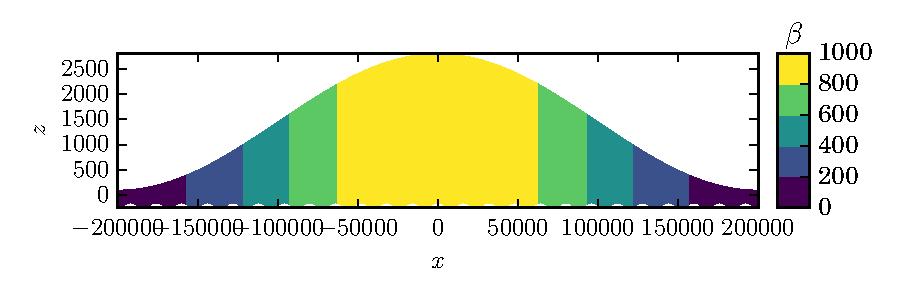
\includegraphics[width=\linewidth]{images/tmc/plane_strain/zero_energy/beta.pdf}
  \caption[Plane-strain TMC example basal traction field]{The basal traction $\beta$ used for the TMC-simulation.}
  \label{tmc_beta_image}
\end{figure}

\pythonexternal[label=cslvr_tmc_plane_strain, caption={\CSLVR script which performs the plane-strain TMC simulation of \S \ref{ssn_tmc_plane_strain_simulation}.}]{scripts/tmc/plane_strain_tmc.py}

\pythonexternal[label=cslvr_tmc_plane_strain_dv, caption={\CSLVR script which plots the result generated by Code Listing \ref{cslvr_tmc_plane_strain}.}]{scripts/tmc/plot_ps_tmc.py}

\begin{figure*}
  \centering
    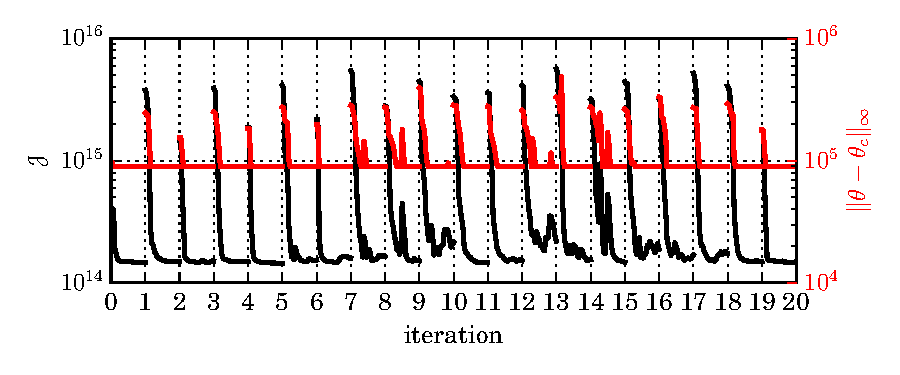
\includegraphics[width=\linewidth]{images/tmc/plane_strain/opt_convergence.pdf}
    \caption[Plane-strain water-optimization convergence diagram]{Objective functional values (\ref{energy_objective}) for each iteration of Algorithm \ref{tmc} (left axis, black) and misfit between the critical value of current energy value $\theta$ and the critical energy value $\theta_c = \theta + W_c L$ (right axis, red) for the $F_b$-optimization procedure of \S \ref{ssn_water_content_optimization}.}
  \label{opt_convergence_image}
\end{figure*}
    
\begin{figure*}
  \centering
    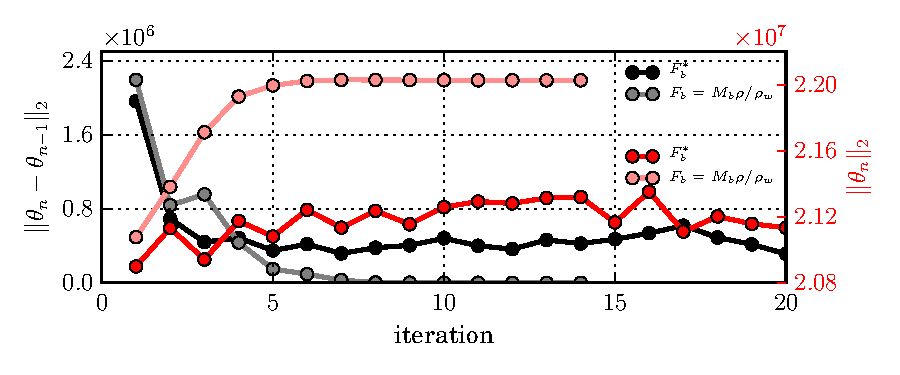
\includegraphics[width=\linewidth]{images/tmc/plane_strain/tmc_convergence.pdf}
    \caption[Plane-strain TMC convergence diagram]{Convergence plot of TMC algorithm \ref{tmc} applied to the plane-strain simulation using both the zero-energy-basal-boundary condition (\ref{zero_basal_water_discharge}) corresponding with $F_b = M_b \rho/\rho_w$ (left axis, grey), and the $F_b$-optimization procedure of \S \ref{ssn_water_content_optimization} using basal-water-discharge-boundary condition (\ref{energy_flux}) (left axis, black).  Also shown is the norm of the current energy guess $\theta_n$ for the zero-energy-basal-boundary condition simulation (right axis, pink) and the $F_b$-optimization procedure simulation (right axis, red).} 
  \label{tmc_convergence_image}
\end{figure*}

\begin{figure*}
  \centering

    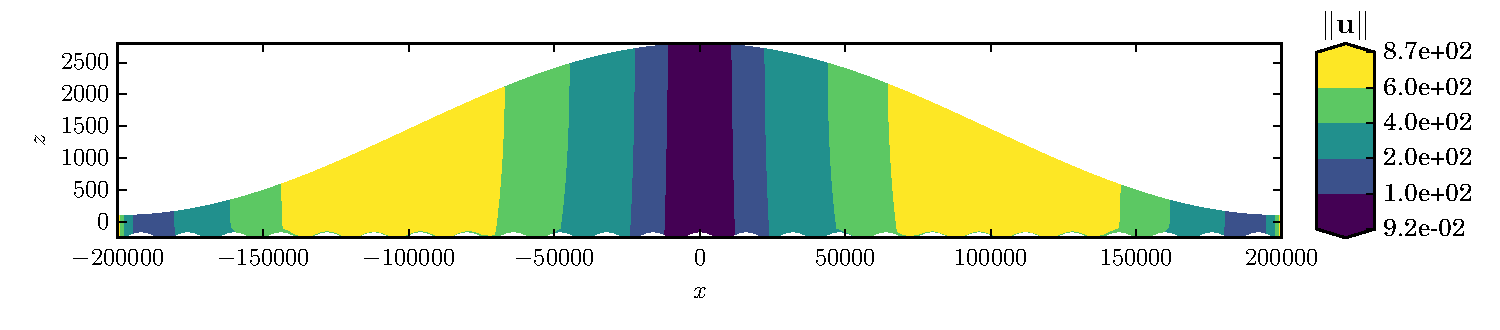
\includegraphics[width=\linewidth]{images/tmc/plane_strain/zero_energy/U_mag.pdf}
    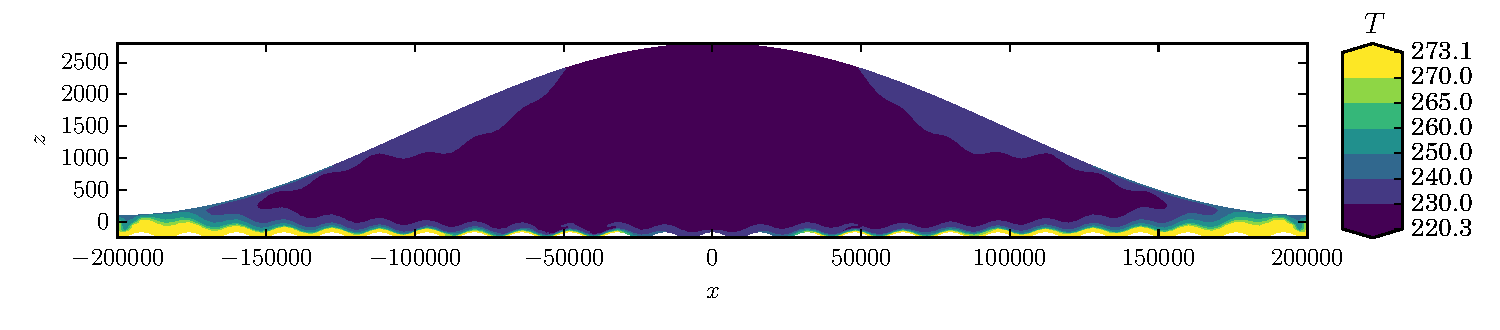
\includegraphics[width=\linewidth]{images/tmc/plane_strain/zero_energy/T.pdf}
    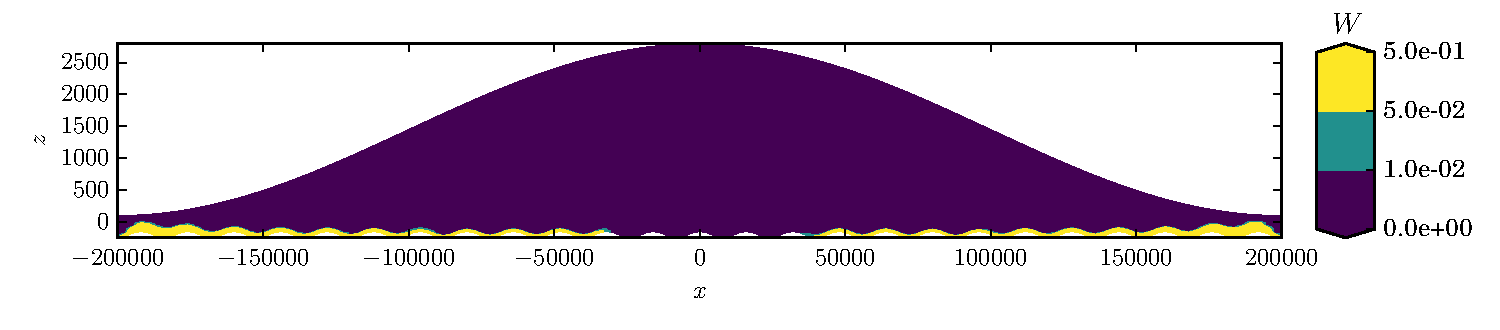
\includegraphics[width=\linewidth]{images/tmc/plane_strain/zero_energy/W.pdf}
    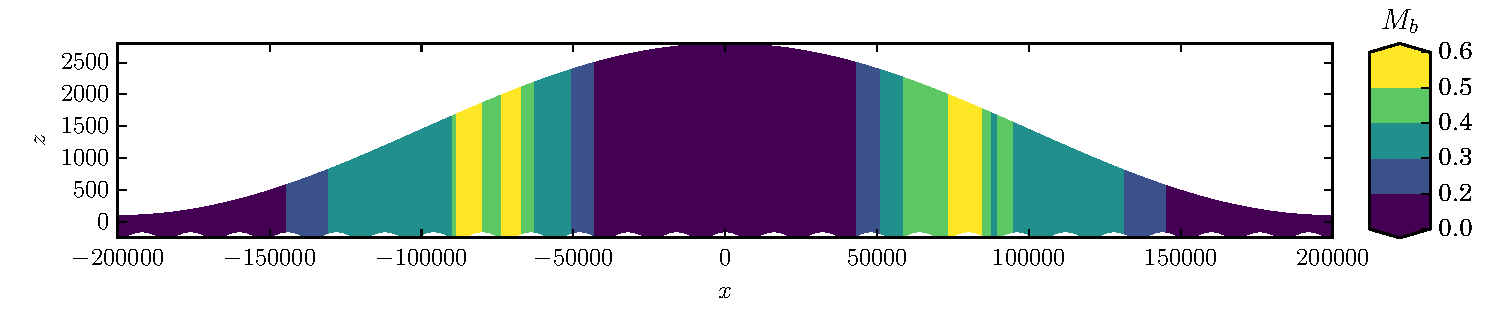
\includegraphics[width=\linewidth]{images/tmc/plane_strain/zero_energy/Mb.pdf}
    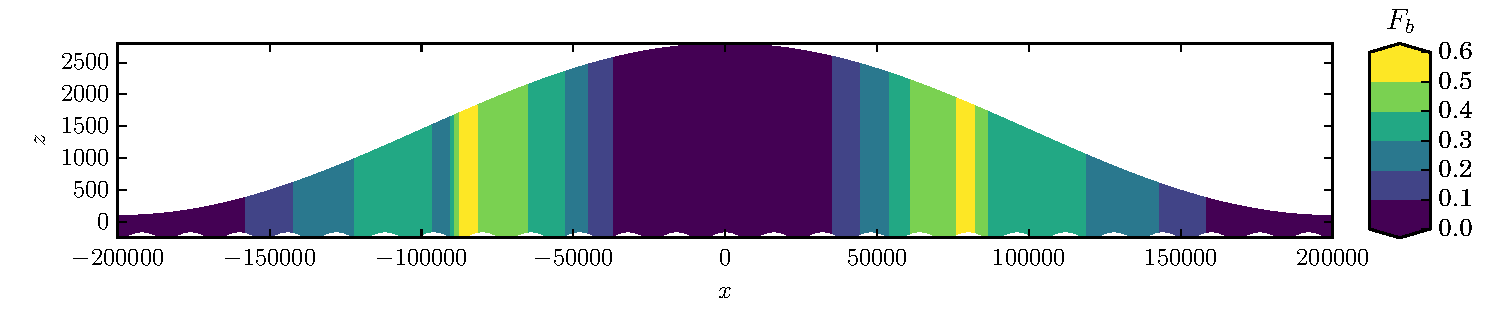
\includegraphics[width=\linewidth]{images/tmc/plane_strain/zero_energy/Fb.pdf}

  \caption[Plane-strain zero-energy-flux solution]{The plane-strain results attained using zero-temperate-energy-flux boundary condition (\ref{zero_basal_water_discharge}).  From top to bottom: velocity magnitude $\Vert \rankone{u} \Vert$, temperature $T$, water content $W$, basal melt rate $M_b$, and basal water discharge $F_b$.}
  \label{tmc_zero_energy_image}
\end{figure*}

\begin{figure*}
  \centering

    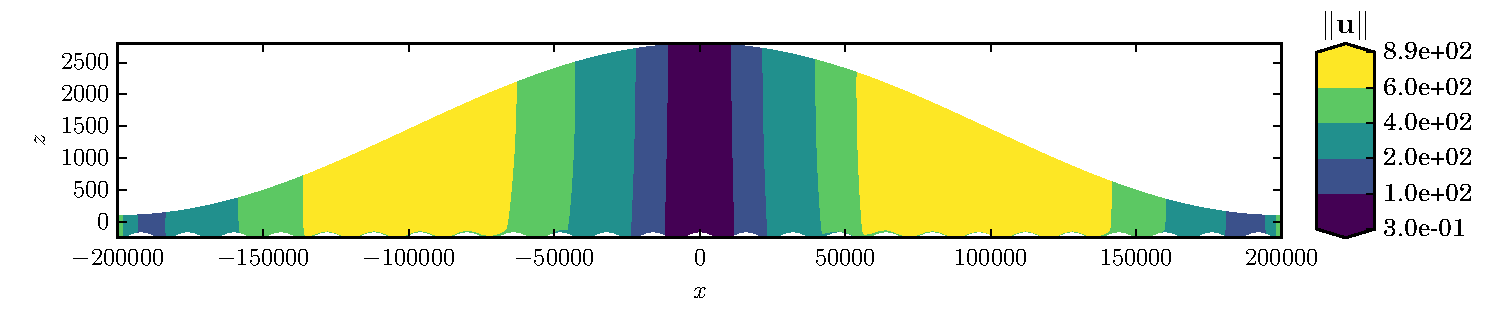
\includegraphics[width=\linewidth]{images/tmc/plane_strain/Fb/U_mag.pdf}
    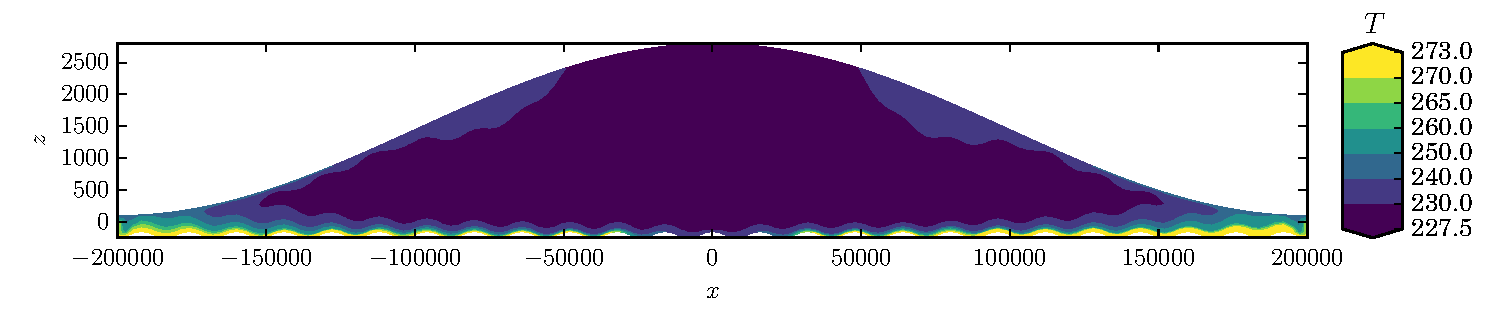
\includegraphics[width=\linewidth]{images/tmc/plane_strain/Fb/T.pdf}
    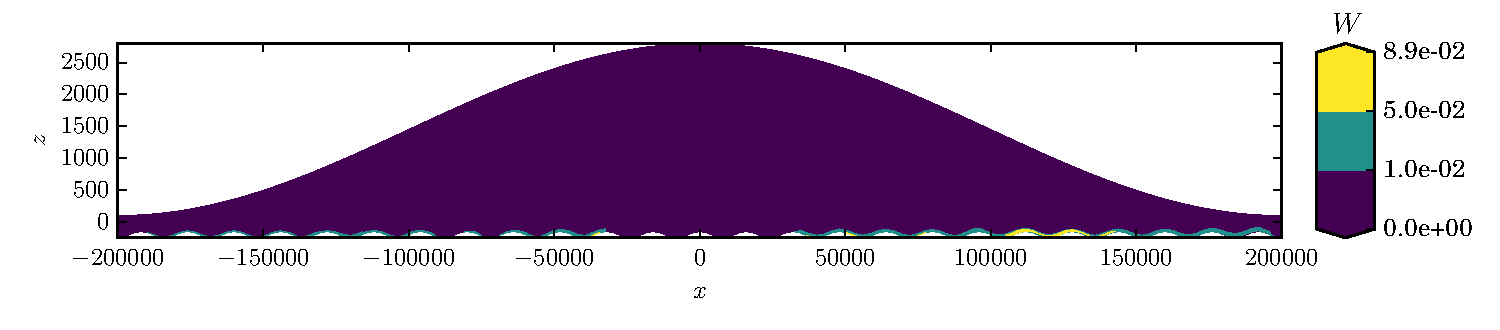
\includegraphics[width=\linewidth]{images/tmc/plane_strain/Fb/W.pdf}
    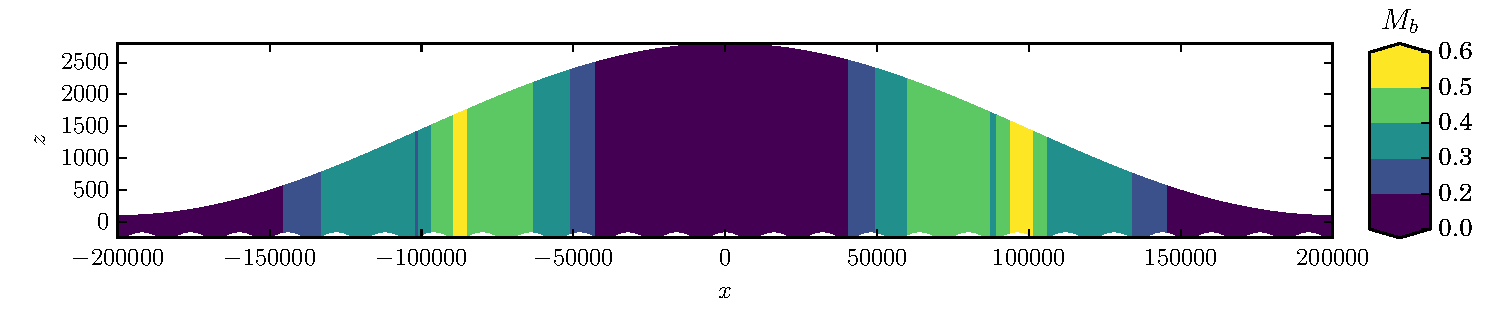
\includegraphics[width=\linewidth]{images/tmc/plane_strain/Fb/Mb.pdf}
    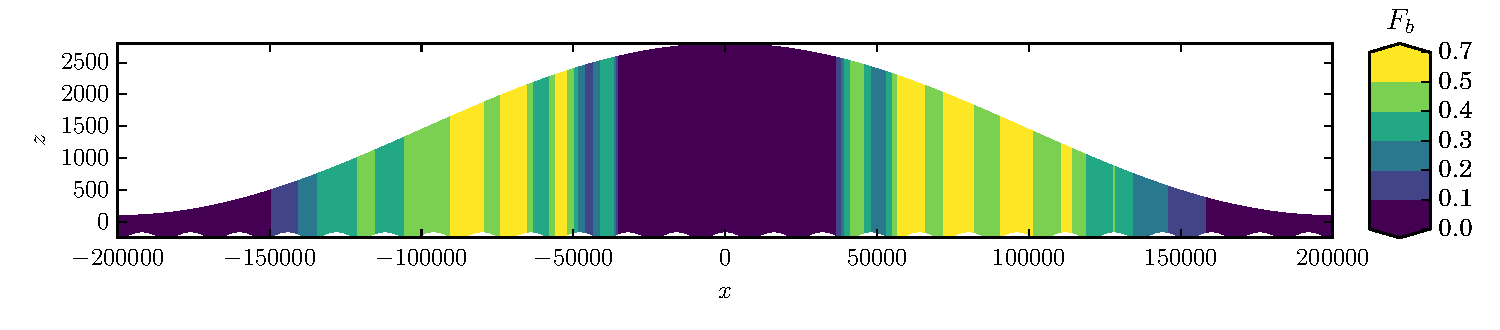
\includegraphics[width=\linewidth]{images/tmc/plane_strain/Fb/Fb.pdf}

  \caption[Plane-strain water-optimization solution]{Plane-strain results attained using the $F_b$ optimization process of \S \ref{ssn_water_content_optimization} with boundary condition (\ref{energy_flux}).  From top to bottom: velocity magnitude $\Vert \rankone{u} \Vert$, temperature $T$, water content $W$, basal melt rate $M_b$, and basal water discharge $F_b$.}
  \label{tmc_Fb_image}
\end{figure*}
